Как было рассмотрено ранее, наличие электрического поля, приложенного
к пьезоэлектрическому кристаллу, вызывает изменение межплоскостного расстояния.
Таким образом, был измерен угловой сдвиг КДО рефлексов (рис. \ref{ris:d11_experiment}), и на основании выражения
 (см. \ref{eq:piezomodule_l}) был рассчитан модуль d11 для кристалла LGT.

\begin{figure}[H]
  \centering
  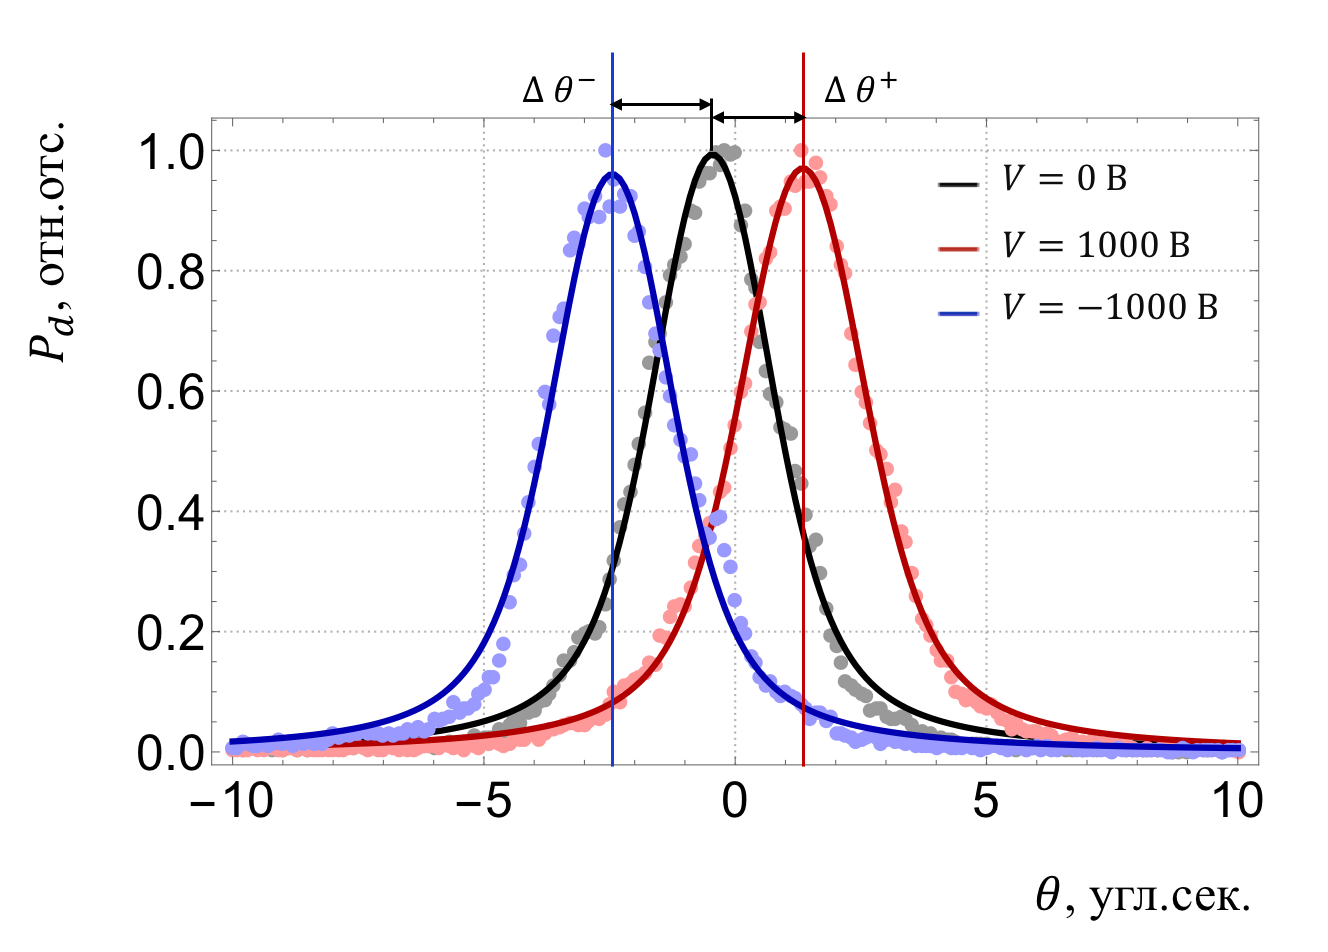
\includegraphics[width=0.7\textwidth]{images/peak_shift_1000v.png}
  \caption{Угловой сдвиг двухкристальной КДО (эксперимент). Кристалл-монохроматор: Si(440),
  кристалл-образец: LGT(440), толщина кристалла $l = 0.27мм$ }
  \label{ris:d11_experiment}
\end{figure}

Экспериментальное определенное изменение брэгговского угла в результате воздействия
электрического поля напряженностью 3,7 кВ/мм составляет 1.89 угл.сек. Таким образом,
наблюдается хорошее соответствие измеренного методом двухкристальной дифрактометрии,
 пьезомодуля $d11 = (6.8 \pm 0.3 ) 10^{-12}$ данным, полученными
  нерентгеновскими методами \cite{LGT_piezo_d11}. В перспективе
  планируется разработка алгоритма восстановления полной матрицы пьезомодулей
  по данным рентгеновской дифрактометрии путем решения системы уравнений, связывающих все $N$
  элементов матрицы пьезомодулей с экспериментально определенными сдвигами КДО для
  такого же количества $N$ рефлексов.
